\documentclass[aspectratio=169]{beamer} % dvipsnames gives more built-in colors
\usepackage{graphicx} % Required for inserting images
\usepackage{transparent}
\usepackage{float}
\usepackage{tikz}
\usepackage{amsmath}
\usepackage[font=scriptsize,labelfont=bf]{caption}
\usepackage{algorithmicx}
\usepackage{listings}
\usepackage{animate}
\usepackage{CJKutf8}
\usepackage{subfiles}
\renewcommand{\footnotesize}{\tiny}

\usepackage{tikz}
\usepackage{tikz-cd}
\tikzcdset{scale cd/.style={every label/.append style={scale=#1},
    cells={nodes={scale=#1}}}}
 
\usepackage{siunitx}  
\sisetup{locale = DE}
\usepackage{multicol}
\usepackage{listings}
\usetikzlibrary{arrows.meta, angles, quotes, calc}

%\usepackage[sorting=none]{biblatex}structuring large files
\usepackage[german=guillemets]{csquotes}
\setquotestyle{english}
%\addbibresource{bibliography.bib}

\usetheme{ufr}
\usecolortheme{ufr}

\newcommand{\bC}{\mathbb{C}}
\newcommand{\bD}{\mathbb{D}}
\newcommand{\bS}{\mathbb{S}}

\newcommand{\mY}{\mathcal{Y}}

\title{What you needa know about Yoneda}
\author{Emma Bach (she/her)}
\date{Seminar on Functional Programming and Logic, Summer Semester 2025}

\begin{document}
%\usebackgroundtemplate{
%        \transparent{0.1}
%        \hspace{7cm}
%        
\includegraphics[width=0.7\paperwidth]{logos/ufr-siegel-grey.png}
%        }

\begin{frame}[plain]
    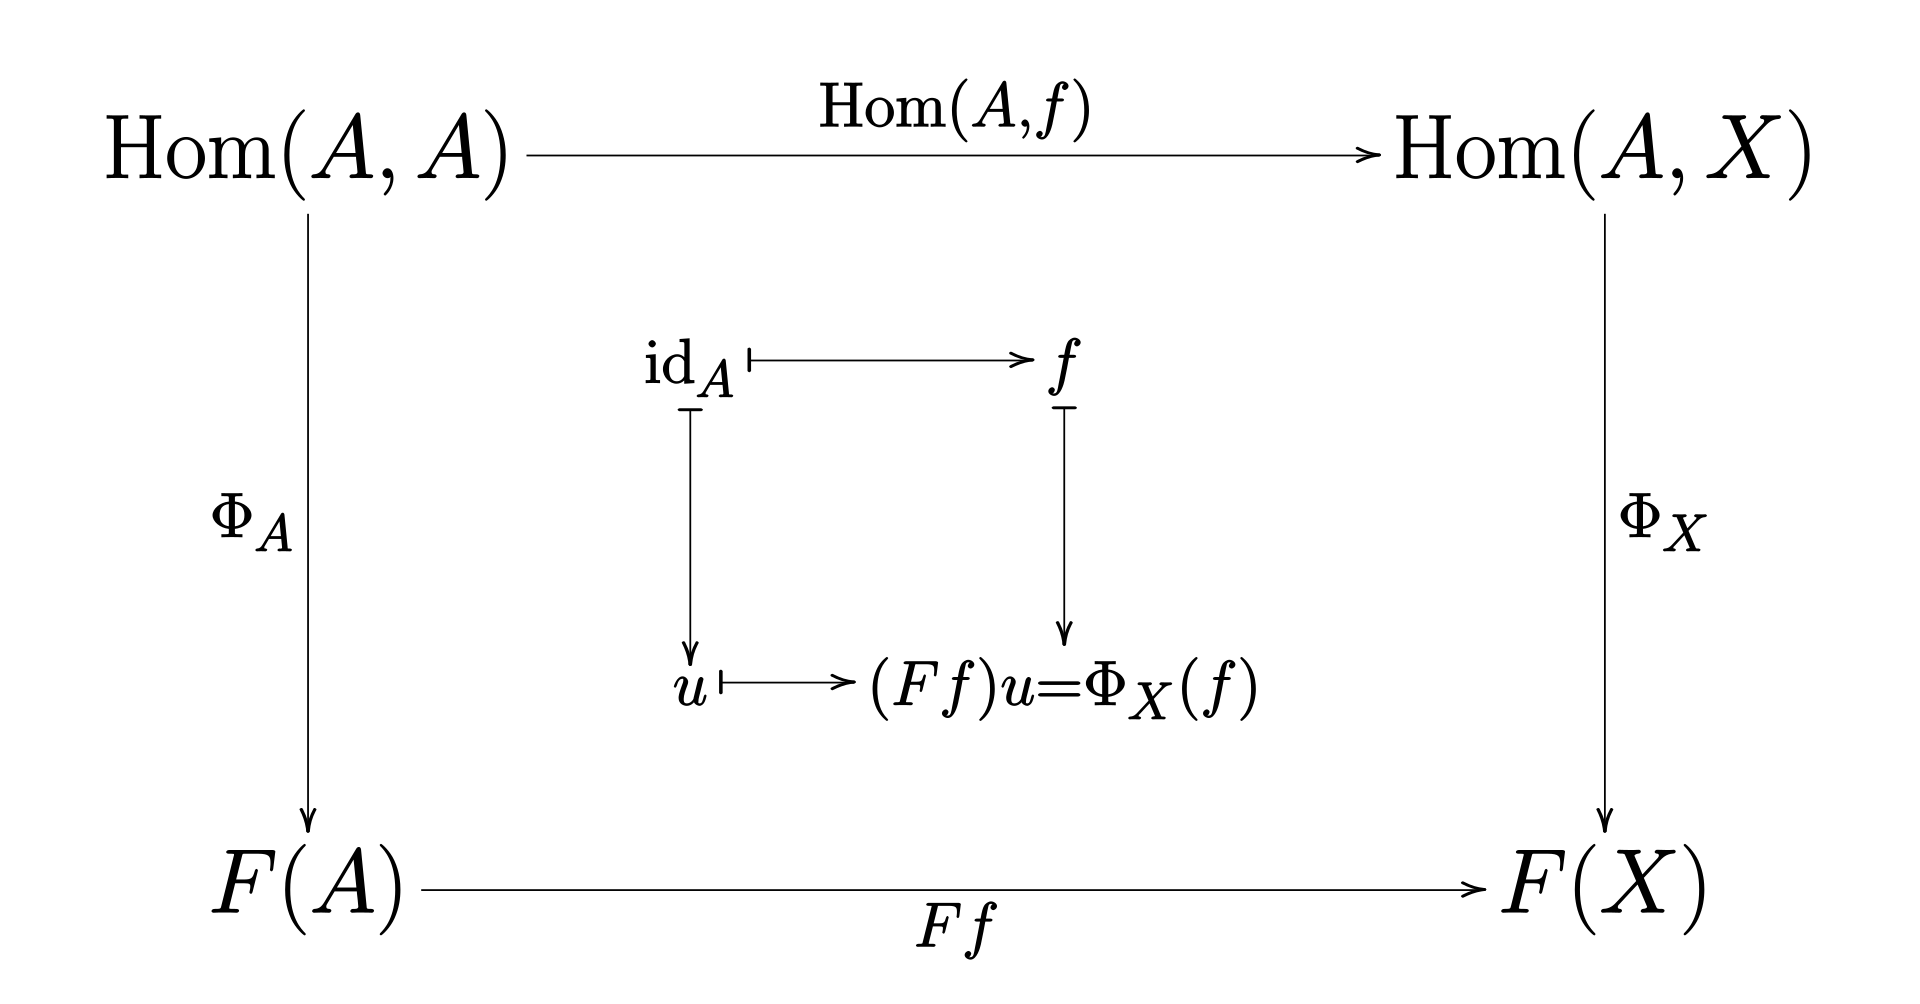
\includegraphics[width=0.4\paperwidth]{figures/Yoneda_lemma_cd.svg.png}
    \titlepage
\end{frame}

%\subfile{sections/basics}
%\subfile{sections/polymorphism}

\begin{frame}[fragile]{The Yoneda Embedding}
\begin{columns}
\column{0.3\textwidth}
\[\begin{tikzcd}
	A && B \\
	\\
	{\mathbb{C}(A, -)} && {C(B,-)}
	\arrow["{f\ \in\ \mathbb{C}(A,B)}", from=1-1, to=1-3]
	\arrow["{\mathcal{Y}}"', dotted, leftrightarrow, from=1-1, to=3-1]
	\arrow["{\mathcal{Y}}", dotted, leftrightarrow, from=1-3, to=3-3]
	\arrow["{\mathcal{Y}(f)}"', from=3-1, to=3-3]
\end{tikzcd}\]
\column{0.7\textwidth}
 \begin{itemize}
    \item Remember that the goal is finding out everything about an object $A$ through its relations to other objects.
    \pause\item So we want a correspondence between objects and their homsets.
    \pause\item Formally, we want a bijective functor
    \begin{align*}
     \mY : \bC &\to \bS et^\bC\\
           A &\mapsto \bC(A,-)
    \end{align*}
    \vspace{-16pt}\pause\item We call $\mY$ the \textit{Yoneda Embedding}.
    \pause\item Given $f \in \bC(A,B)$, $\mY(f)$ is a morphism between $\bC(A, -)$ and $\bC(B, -)$ in the functor category $\bS et^{\bC}$.
    \pause\item Therefore, $\mY(f)$ is a natural transformation between $\bC(A, -)$ and $\bC(B, -)$
 \end{itemize}
\end{columns}
\end{frame}

\begin{frame}{The Yoneda Lemma}
    \begin{itemize}
        \item It turns out we can do even better!
        \pause\item We can construct the set of all natural transformations between $\bC(A, -)$ and \underline{any} Functor $F :\bC \to \bS et$.
        \pause\item Specifically, the Yoneda Lemma states that:
        \begin{align*}
          \text{Nat}(\bC(A,-), F) \simeq F(A))
        \end{align*}
        \begin{itemize}
          \vspace{-18pt}\pause\item Furthermore, this isomorphism is a natural transformation.
          \pause\item So we can construct a unique $\mY$ with our desired properties from any element $F(A)$.
          \pause\item Vice versa, if we know all natural transformations $\text{Nat}(\bC(A,-), F)$, we can construct the set $F(A)$.
        \end{itemize}
    \end{itemize}
\end{frame}

%\subfile{sections/applications}
\end{document}
